\chapter{Implementation}

Implementation of designs has taken place step by step following the timeline plans and wireframe diagrams to achieve the desired output on screen. 
The implementation phase of the project involves the execution of below tasks in an organized way. \newline
\textbf{Tasks Planned for Execution:}
    \begin{enumerate}
        \item Authentication
        \item News Data Script
        \item Access News feed
        \item Contextual Personalization Implementation
        \item Behavioral Personalization Implementation
        \item Visualization and Projections
        \item Recommendation thoughts and concepts
        
    \end{enumerate}
\textbf{Authentication:} \newline
Springboot authentication is performed using spring security with \textbf{UsernamePasswordAuthenticationFilter} which is implemented using \textbf{WebSecurityConfigurerAdapter}. \\
Code snippet for spring security which is implemented inside configure method:  \newline

 \begin{figure}[h!]
     \begin{center}
    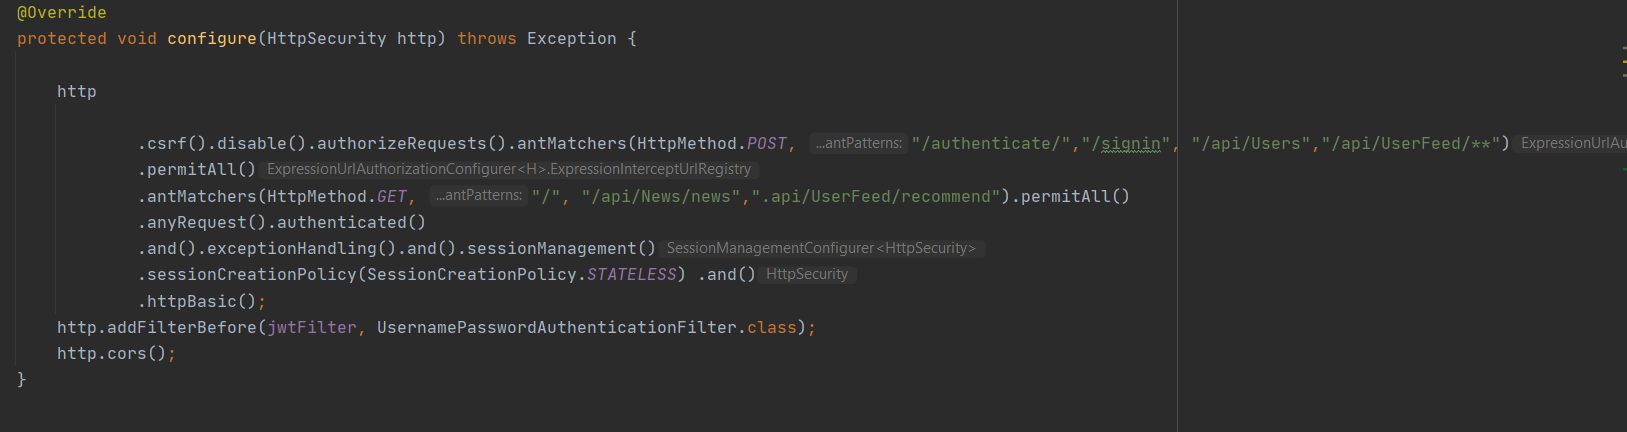
\includegraphics[width = \linewidth]{images/security.PNG} 
  \end{center}
\centering \caption{Spring Security}
\end{figure}

\textbf{News Data Script:} \newline
    News data is loaded into database from the api json response using the \textbf{jackson-databind} dependency in springboot. We will read the DeatiledNews.json and map the news to our NewsApi model. This way we can map set of news data to our News Model.
    
    
\begin{figure}[h!]
     \begin{center}
    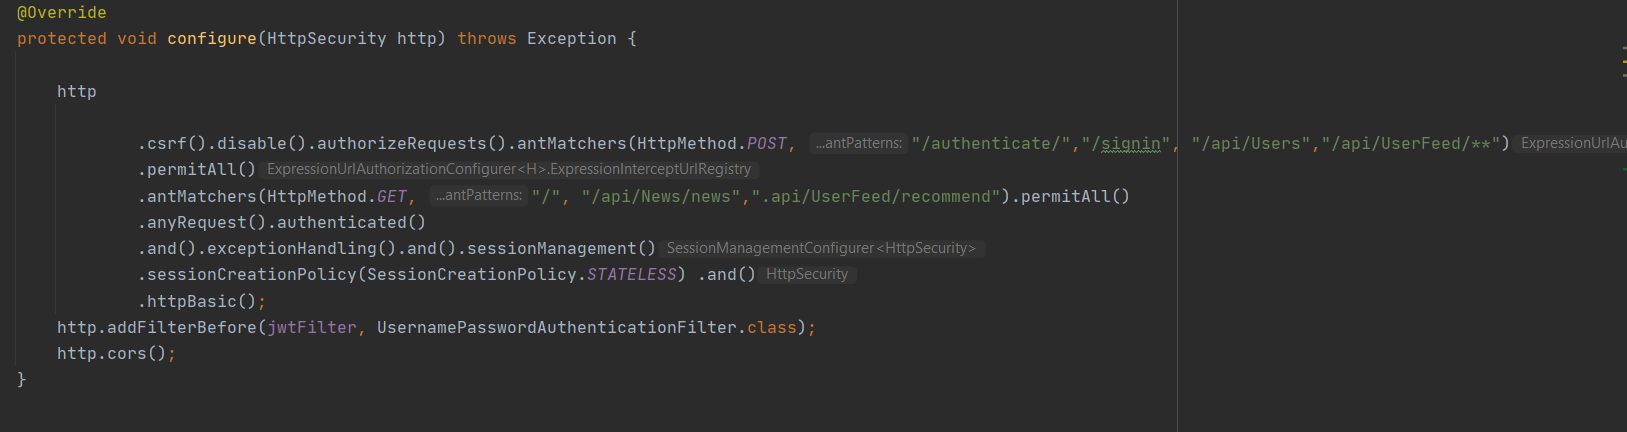
\includegraphics[width = \linewidth]{images/security.PNG} 
  \end{center}
\centering \caption{Spring Security}
\end{figure}

\textbf{ Access News feed: } \newline
News Feed data can be accessed by any user who land on the application url and does not require any login to read the news.
News data is accessed with or without parameters country and category based on requirement to get the desired news using the \textbf{@GetMapping} Rest call with no authorization header for general news to allow access for all readers. For specific category or country news by any user, the use of http authorization header with bearer tokens becomes necessary.

   
\begin{figure}[h!]
     \begin{center}
    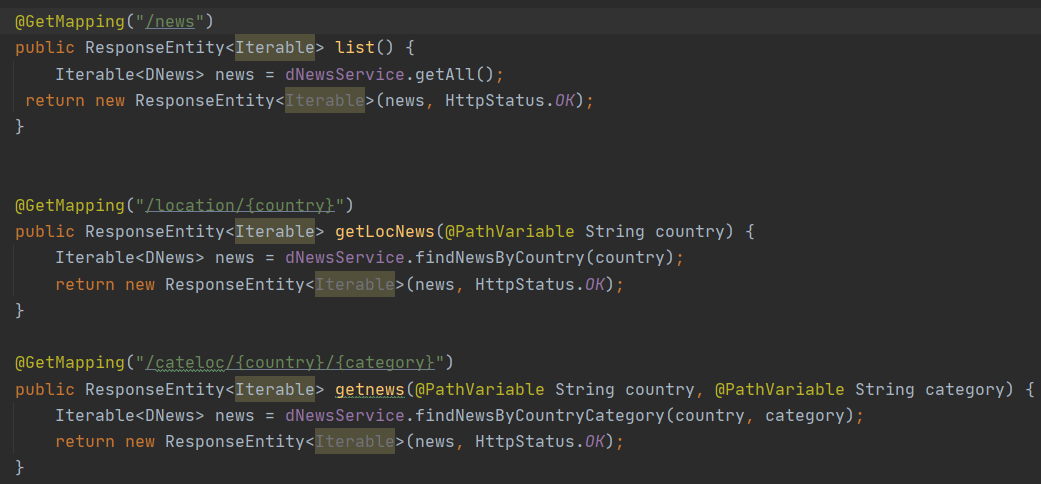
\includegraphics[width = \linewidth]{images/AccessNews.PNG}s 
  \end{center}
\centering \caption{News Feed}
\end{figure}

 
\textbf{Contextual Personalization Implementation :}\newline
Contextual Personalization is implemented using user details which are provided during the signup. 
For the initial prototype I have taken the user selected preferences and the location for providing personalization.\newline
\textbf{Selected Preferences}\newline
The user preferences are taken into account when each user is being added to the user database and their category map is setup with the standard initial weight which is assigned +2. The weight is chosen by the developer as a standard for the application.\newline

 \begin{itemize}
     

 \item \textbf{Zonal News}\newline
Location is considered while providing the personalization and to make it more lively the user's location news is made available with visualization setup using amcharts which provides geographical geojson data and map to load all the country details and load respective data based on selection. 
And the users are provided options to filter any category data upon country selection. This helps in filtering and learning any specific news for any country to understand the zonal news much better.

 \item \textbf{Implementation with Amcharts and BehaviorSubject:}\newline
Amcharts are implemented using some basic scripts from amcharts.com and enhanced with BehaviorSubject to store any value and  return immediately on subscription.
This is helpful in holding the category selection while switching to any other country and return the previously help category data for the selected country.

  
\begin{figure}[h!]
     \begin{center}
    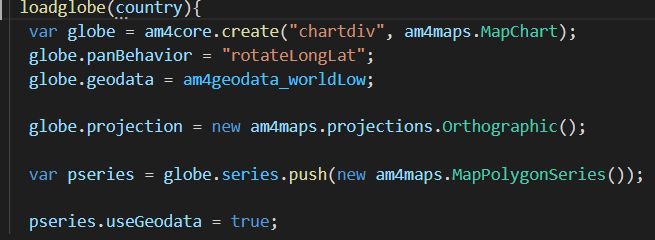
\includegraphics[width = \linewidth]{images/amchartsglobe.PNG}s 
  \end{center}
\centering \caption{Amcharts Visualization}
\end{figure}
 \end{itemize}
 
 
\textbf{Behavioral Personalization Implementation: }\newline
Behavioral Personalization is implemented by tracking user interactions with \textbf{weight-map algorithm} which assigns respective assigned weights for various reactions and measures their interests based on varying weights. \newline

\textbf{How it works?}
The different category news are added or reduced based on users changing interests everytime and their userfeed is filled with respective number of news data. More the interests towards a category, more the number of those news data and vice-versa. \newline
There are various methods which works for every user interactions like add to favorites, likes, save feeds and updates the user interests everytime through the user-category map. Then finally the user feed is fetched using \textbf{FetchByUid} which loads respective number of data based on interests neither more nor less.
The entire logic goes inside the back-end  Controller and Service domains- 'UserFeedController' and 'UserFeedService' classes. \newline


\textbf{Visualization and Projection}
Visualization and projection of user charts using amcharts works with the defined user-category map where each user holds a map with category name and respective weights where the weights gets updated with personalization aspects based on the Weight-Map Algorithm. 
The data is projected with pie-charts in-built chart data with values filled from user map and the code snippet for pie-chart projection looks like :

\begin{figure}[h!]
     \begin{center}
    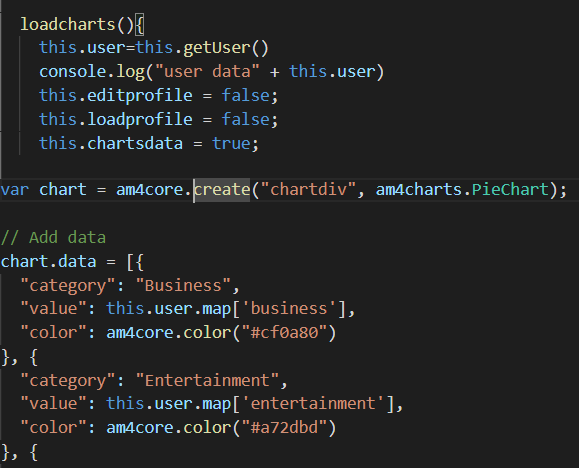
\includegraphics[width = \linewidth]{images/chartdata.PNG}s 
  \end{center}
\centering \caption{Chart Projection}
\end{figure}

\textbf{ Recommendation thoughts and concepts: }
 Recommendation works based on conceptual Machine learning algorithmic implementation. The recommendation algorithm is implemented by Mahout Recommendation system which is used in this application to gather the interests and preferences of various users and match them based on their similarity of interests and provide various categories which might be preferred by the users who might haven't gone through those news categories before. This is the logical working process of \textbf{User based Similarity} which suggests users based on similar taste.
 
\textbf{ Mahout Recommendation System: } 
The algorithm works very well 